\subsection{Building complex Decision Boundaries}
We'll denote a neuron with $n$ inputs as $f_n$ i.e. $f_n:\re^n \to \{0, 1\}$ and $f_n$ is designed using weight $\wb \in \re^n$ and bias $b$. For $\mx \in \re^n$,
\begin{equation*}
f_n(\mx) = \mathbbm{1}_{\{\wb^T\mx + b > 0\}}
\end{equation*}
For the below problems we'll ignore classifying on exactly the Decision Boundary.

\begin{enumerate}[label=\alph*)]
\item Using a single neuron, implement the the OR and AND gates i.e. when $\mx \in \{0, 1\}^n$, $f_n(\mx)$ should output the corresponding boolean logic.



\item Realize that using a single neuron, $f_n$ you can implement every possible linear decision boundary in $\re^n$. Note that for a single geometric hyperplane in $\re^n$, there are two possible decision boundaries (See \autoref{fig:linear1} and \autoref{fig:linear2}).

\item If you want to partition $\re^2$ into different regions using straight lines, each classified as one of $\{0, 1\}$, you can draw these lines and use boolean logic to model on which side a point in $\re^2$ lies w.r.t each line (one of $\{0, 1\}$). Taking ideas from the above parts, draw a $2$ Layer network with atmost $3$ neurons that can draw every decision boundary shaped like \autoref{fig:parallel} and \autoref{fig:tri}. Can the same network be use to draw decision boundaries \autoref{fig:linear1} and \autoref{fig:linear2}. Can this network draw \autoref{fig:cross}?


\item Show why you can't implement the XOR gate using a single neuron. Now, use two layers of neurons (atmost $3$ neurons in total) to implement XOR, in case of $\mx \in \{0, 1\}^2$.

\item Using atmost $3$ layers and $5$ neurons, implement all decision boundaries like \autoref{fig:cross}. Will this also represent all decision boundaries \autoref{fig:linear1} through \autoref{fig:cross}.

\item Think about the minimum number of layers and neurons needed to implement any boolean function of $n$ variables. Using the ideas above, can you design a Neural Network that can perfectly classify a $m$ points in $\re^2$, without knowing their positions and labels beforehand.
\end{enumerate}

\begin{figure}[H]
    \centering
    \begin{minipage}{0.45\textwidth}
        \centering
        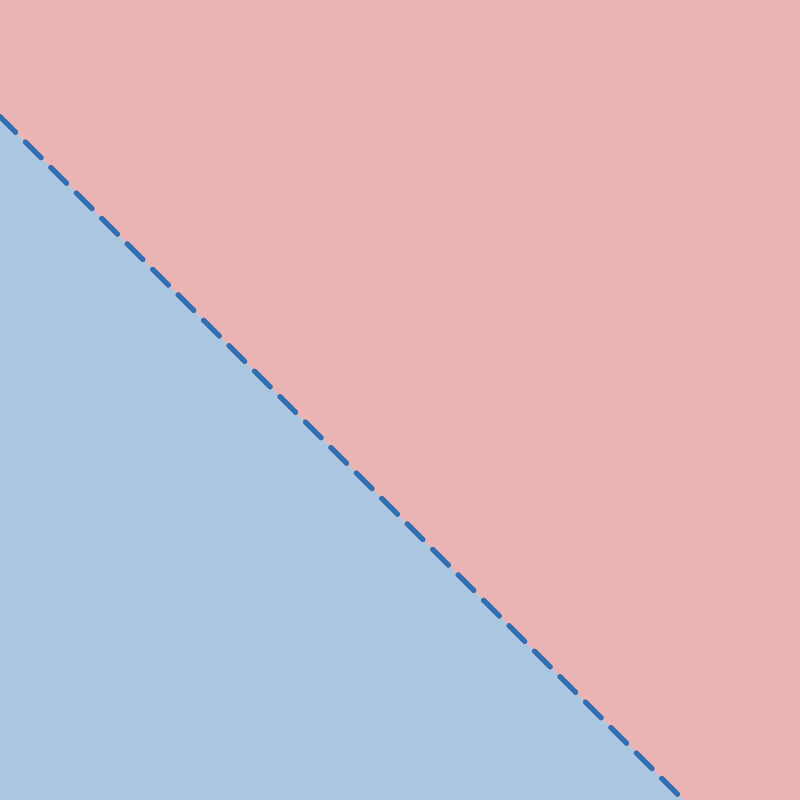
\includegraphics[width=\textwidth]{images/boundaries/linear1.png}
        \caption{Boundary 1}
        \label{fig:linear1}
    \end{minipage}
    \hfill
    \begin{minipage}{0.45\textwidth}
        \centering
        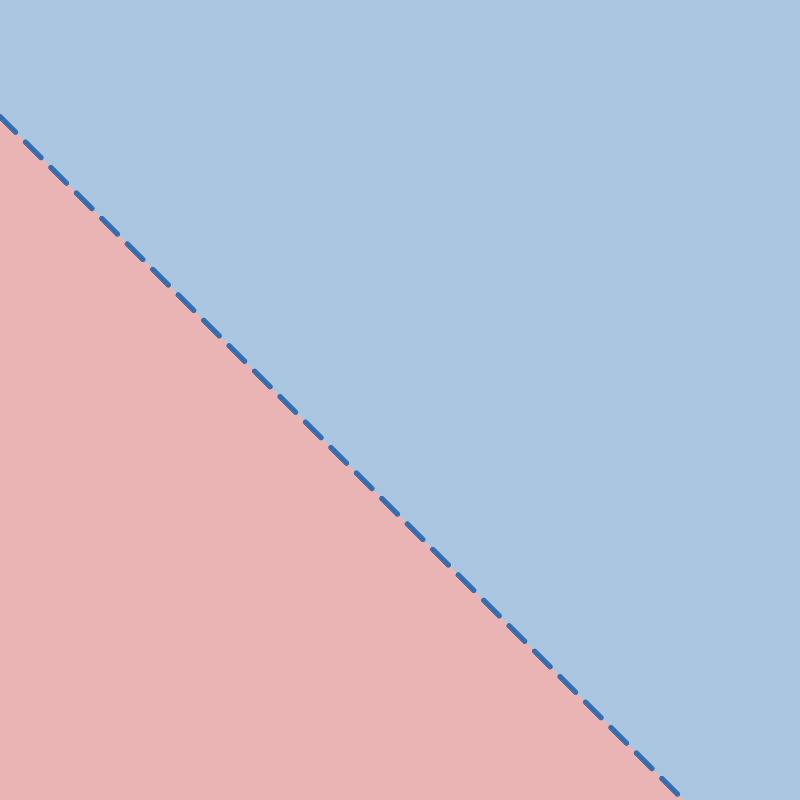
\includegraphics[width=\textwidth]{images/boundaries/linear2.png}
        \caption{Boundary 2}
        \label{fig:linear2}
    \end{minipage}
    
    \vspace{0.5cm} 
    
    \begin{minipage}{0.45\textwidth}
        \centering
        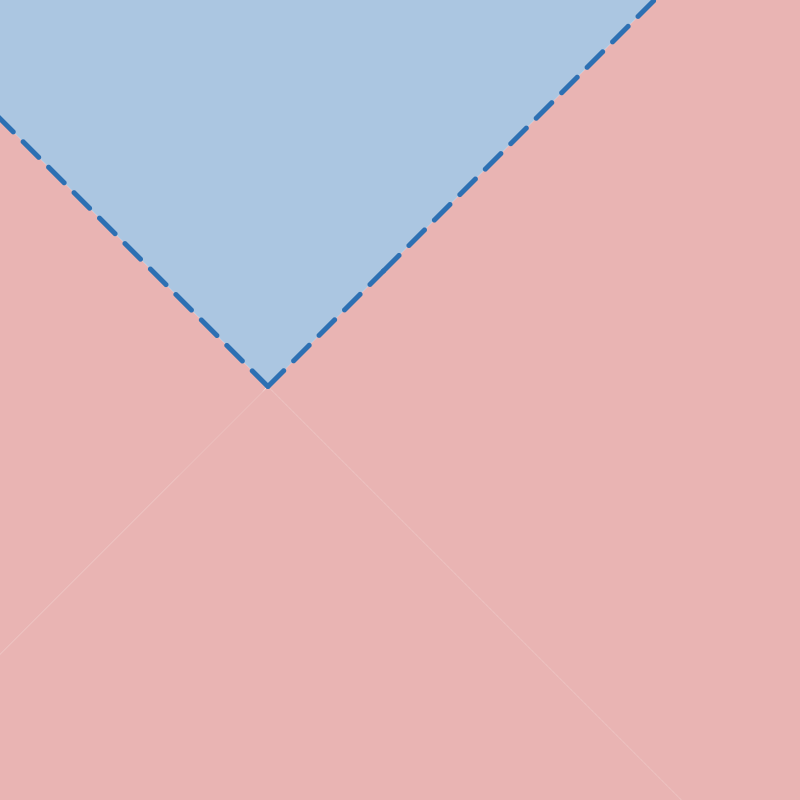
\includegraphics[width=\textwidth]{images/boundaries/tri.png}
        \caption{Boundary 3}
        \label{fig:tri}
    \end{minipage}
    \hfill
    \begin{minipage}{0.45\textwidth}
        \centering
        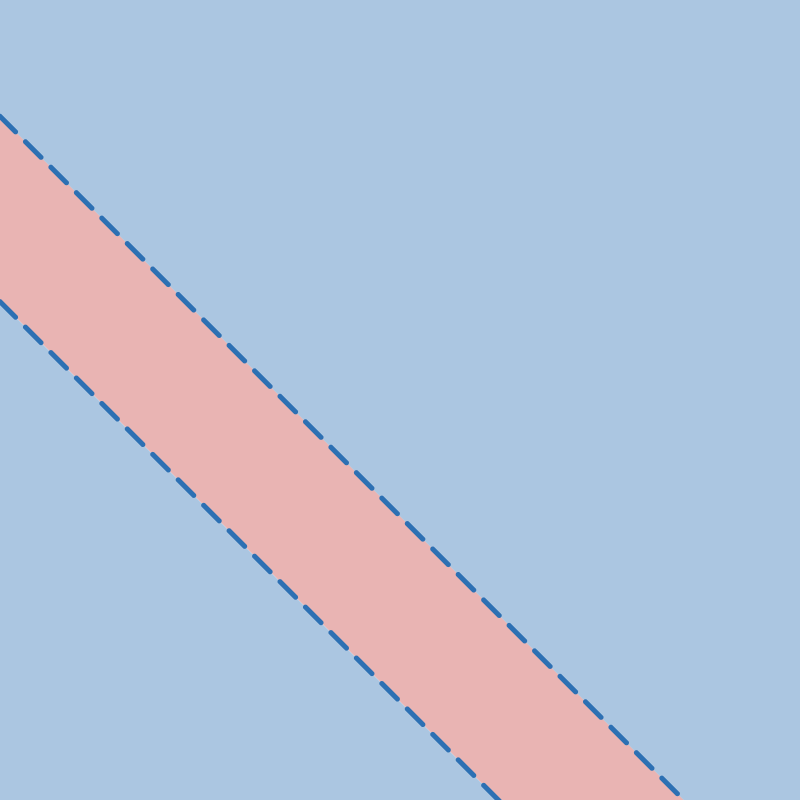
\includegraphics[width=\textwidth]{images/boundaries/parallel.png}
        \caption{Boundary 4}
        \label{fig:parallel}
    \end{minipage}

\end{figure}

\begin{figure}[H]
    \centering
    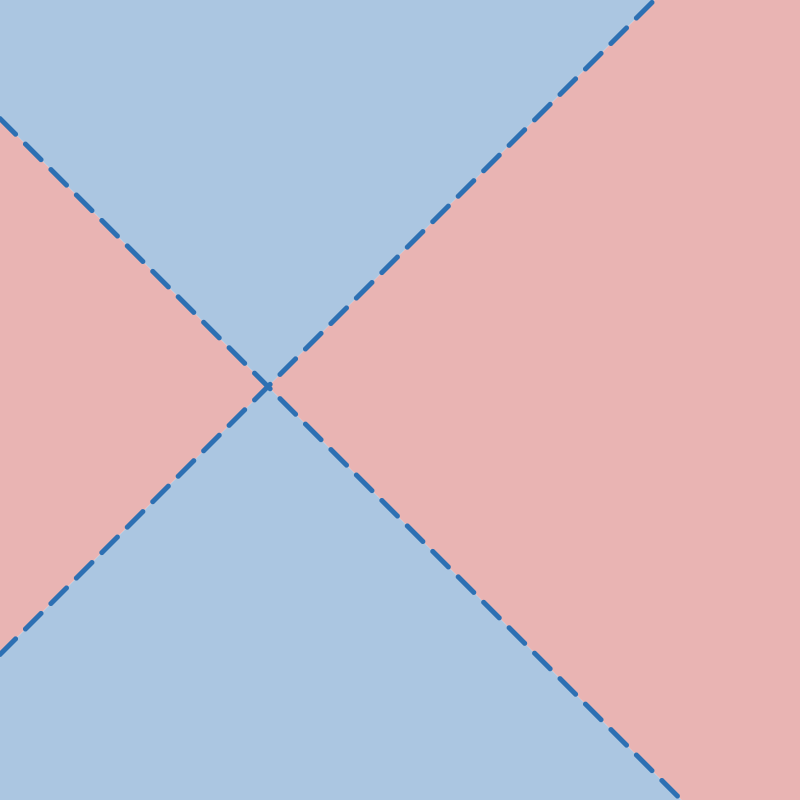
\includegraphics[width=0.75\textwidth]{images/boundaries/cross.png}
    \caption{Boundary 5}
    \label{fig:cross}
\end{figure}